\documentclass[dvipdfmx]{jarticle}
\usepackage{graphicx}
\usepackage[top=30truemm,bottom=30truemm,left=25truemm,right=25truemm]{geometry}
\usepackage{listings,jvlisting}
\usepackage{url}

\lstset{
  basicstyle={\ttfamily},
  identifierstyle={\small},
  commentstyle={\smallitshape},
  keywordstyle={\small\bfseries},
  ndkeywordstyle={\small},
  stringstyle={\small\ttfamily},
  frame={tb},
  breaklines=true,
  columns=[l]{fullflexible},
  numbers=left,
  xrightmargin=0zw,
  xleftmargin=3zw,
  numberstyle={\scriptsize},
  stepnumber=1,
  numbersep=1zw,
  lineskip=-0.5ex
}

\makeatletter
\newcommand{\subsubsubsection}{\@startsection{paragraph}{4}{\z@}%
  {1.0\Cvs \@plus.5\Cdp \@minus.2\Cdp}%
  {.1\Cvs \@plus.3\Cdp}%
  {\reset@font\sffamily\normalsize}
}
\makeatother
\setcounter{secnumdepth}{4}

\begin{document}
\begin{titlepage}
    \begin{center}
        {\huge 情報科学演習D 課題1レポ―ト}
        \vspace{180pt}\\
        \begin{tabular}{rl}
            氏名 & 山久保孝亮\\
            所属 & 大阪大学基礎工学部情報科学科ソフトウェア科学コース\\
            メールアドレス & u327468b@ecs.osaka-u.ac.jp\\
            学籍番号 & 09B22084\\
            提出日 & \today\\
            担当教員 & 桝井晃基 松本真佑
        \end{tabular}
    \end{center}
\end{titlepage}
\section{システムの仕様}
課題1で作成したプログラムの仕様は以下の通りである.
\begin{itemize}
    \item Pascal風言語で記述されたpasファイルを入力として,字句解析の結果であるtsファイルを出力する.また,開発対象のrunメソッドの第一引数はpasファイル名,第二引数はtsファイル名を指定する.
    \item  正常に処理が終了した場合は文字列"OK"を返し,入力ファイルが見つからない場合は文字列"file not found"を返す.
\end{itemize}
\section{課題達成の方針と設計}
課題1は字句解析と,解析したトークンをそれに対応する文字列とともにtsファイルに書き込む処理に分けられる.
\subsection{字句解析の処理}
字句解析の処理は以下のオートマトンに基づいて開発した.
\begin{figure}[h]
    \centering
    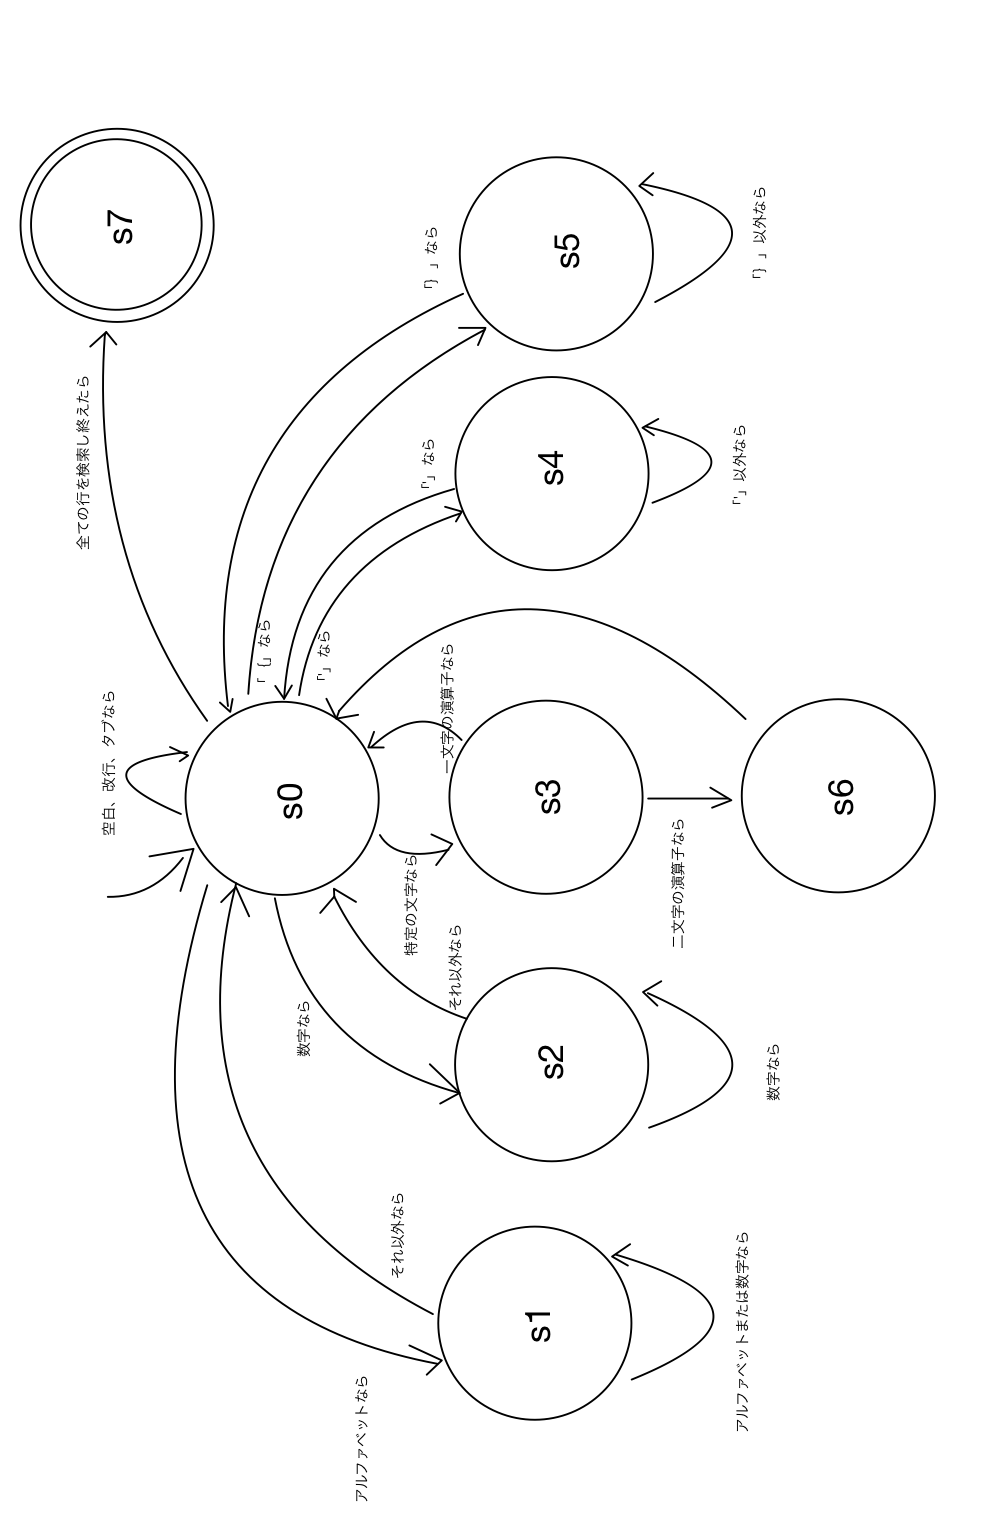
\includegraphics[width = 6cm, angle = -90]{automaton.png}
    \caption{字句解析部分のオートマトン}
\end{figure}
\\このオートマトンは合計8つの状態が存在し,初期状態はs0,受理状態はs7である.それぞれの有効辺の条件分岐は入力されたpasファイルの一文字について判定している.状態が変わるとその次の文字について調べ,pasファイルの最後の文字になると受理状態に遷移する.s1からs0に遷移するとき以外,s0に遷移する際にtsファイルに出力する処理を行う.
\\また,ここではpasファイルの一文字を取り出してそれについて条件分岐を作成しているが,トークンが複数の文字で構成される場合,読み込んだ文字を保存しておく必要がある.そのためにtoken\_loaded\_letterというリストを用意し,
トークンの終わりが確定するまで各文字を記憶しておく.そして確定してから各要素を連結して文字列に変換し,そのリストを初期化する.以降この処理を文字列連結の処理と呼ぶ.
\subsection{tsファイルに書き込む処理}
tsファイルに出力する処理を行うために,ソースコード上の字句,字句解析機上でのトークン名,IDのそれぞれを格納するリストを事前に用意しておく.
具体的には,ソースコード中の字句をtoken,字句解析機上でのトークン名をtoken\_name,IDをtoken\_idというリストを用意しておく.これらのリストの要素の順番はすべて対応している.例えば,token,token\_name,token\_idの0番名にはそれぞれand,SAND,0が格納されているように,それぞれのリストのインデックスに対応する文字列が格納されている.
これによりインデックスのみでトークン名とIDを取り出すことができる.また,divと\textbackslash はどちらも格納し,token\_nameでも同じトークン名で,token\_idでも同じIDで格納した.
\\そして,取り出したトークンがtokenの内の要素と一致するかを判定し,token\_nameとtoken\_idに格納されている対応する文字列を書き込む.また,この処理は2.1のオートマトンのs1以外の状態で処理されるので,同じ記述を繰り返すことを避けるために関数として定義した.
\section{実装プログラム}
2で記述した方針で作成するために,ここではpasファイルから文字を取り出す処理,字句解析のオートマトンのそれぞれの状態の処理,tsファイルへの書き込み処理の3つについて記述する.
\subsection{pasファイルから文字を取り出す方法}
pasファイルから各文字を一字ずつ評価するために,pasファイルから一行ずつ取り出し,各行から一字ずつ取り出す処理を行う.以下はその部分のプログラムを抜粋したものである.
\begin{lstlisting}
final List<String> buffer = Files.readAllLines(Paths.get(inputFileName));
String line = buffer.get(i) + "\n";
while(i<buffer.size()) {
    String line = buffer.get(i) + "\n";
    while(j < line.length()) {
        char c = line.charAt(j);
        j++;
    }			
    i++;
 }
\end{lstlisting}
これによって,cにプログラムの各文字が格納されていくことになる.また,2行目でlineの最後に\textbackslash nを追加しているのは
Files.readAllLines()では改行の文字が含まれないためである.
\subsection{字句解析のオートマトンの処理}
まず図1のオートマトンの各状態に遷移するための条件分岐について記述する.3.1で取得したcについて評価してどの状態に対応するかを判定する.以下はその部分のプログラムを抜粋したものである.
\begin{lstlisting}
    //s0
    if(c == ' ' || c == '\t'|| c == '\n') {
    }else if(c == '{'){//s5
    }else if(c == '\'') {//s4
    }else if("/=<>+-*()[]:;.,".indexOf(c) !=-1){
        if((c == '<'||c == '>'|| c == ':'|| c == '.')&&( j + 1 < line.length())) {//s6
        }else {//s3
        }
    }else if("0123456789".indexOf(c)!=-1 && !loaded_token_letter.isEmpty() && !Character.isAlphabetic(loaded_token_letter.get(0).charAt(0))){//s2
    }else {//s1
    }
\end{lstlisting}
この部分は3.1の二つのwhile文中に記述されているので,pasファイルの文字数分だけ実行される.
5行目と9行目の"文字列".indexOf(c)は文字列中にcが含まれているかどうかを判定しており,これで数字と特定の文字列が含まれているかを判定している.
\\5行目のs3に遷移するかどうかを判定する際の文字列では,指導書の表6のトークン一覧に記載されていた記号を羅列したものであり,図1のオートマトンの特定の文字というのはこの""で囲まれた文字列に対応する.また,6行目のs6に遷移するかどうかを判定する際の文字列では,トークン一覧に記載されていた二文字の演算子の内の一文字目を羅列したものである.
\\9行目のs2に遷移するかを判定する条件文では,取り出した文字が数字であるかだけでなく,切り出し中のトークンの一文字目がアルファベットであるかを判定することで
取り出した数字が符号なし整数の一部なのか,識別子の一部なのかを判定している.また,isEmpty()を使用しているのはloaded\_token\_letterに何も格納されていないにもかかわらず一文字目を調べてしまうことを避けるためである.
\subsubsection{s1の処理}
ここでは,識別子のトークンを切り出す処理を行う.2.1で記述したようにtoken\_loaded\_letterにcをString型に変更して追加する.
この状態に遷移した時点ではトークンの終わりであるかがわからないのでここで書き込みは行わない.
\subsubsection{s2の処理}
ここでは,符号なし整数を切り出す処理を行う.
符号なし整数の終わりは数字ではない文字が来るまでなので,それまでdo-while文を用いて先読みする.この時の条件文は”cが「0から9」に含まれない”である.先読みしている間はそれぞれの文字をloaded\_token\_letterに追加してjをインクリメントしていく.
繰り返しから抜けた際にはjは符号なし整数の最後の数字の次の文字を指しているので,jを一つ減らす.そして文字列連結の処理を行い,writeToken()を呼び出す.writeToken()については3.3で記述する.
このとき,
行番号を表す引数にはi+1を格納する.iではなくi+1を格納するのは,iは0から始まっているため行番号に変換するにはすべて1を足す必要があるためである.
\subsubsection{s3の処理}
ここでは,一文字の演算子のトークンを切り出す処理を行う.まず最初にloaded\_token\_letterに文字列が格納されているかどうかを調べる.
これは,演算子がある時点でそれ以前の文字列がトークンとして確定するためである.そしてs2と同様に書き込みの処理を行う.
\subsubsection{s4の処理}
ここでは,文字列を切り出す処理を行う.文字列の終わりを表す「’」が現れるまでdo-while文を用いて先読みする.この時の条件文は”cが「’」ではない”である.先読みしている間はそれぞれの文字をloaded\_token\_letterに追加してjをインクリメントしていく.
繰り返しから抜けた際にはjは文字列の終わりを表す「’」を指しているので,jに対して変化は加えない.そしてs2と同様に書き込みの処理を行う.
\subsubsection{s5の処理}
ここでは,注釈に対する処理を行う.s4と同様,注釈の終わりを表す「}」が現れるまでdo-while文を用いて先読みする.この時の条件文は”cが「}」ではない”である.注釈の内容は送信しないので,繰り返しの中ではjをインクリメントするだけである.
繰り返しから抜けた際にはjは注釈の終わりを表す「}」を指しているので,jに対して変化は加えない.
\subsubsection{s6の処理}
ここでは,二文字の演算子になり得るトークンを切り出す処理を行う.具体的には,cとは別にnextという変数にcの次の文字を読み込む.これにより,cとnextを合わせて二文字の演算子であるかを判定することができる.
二文字の演算子であればその二つの文字を連結して,一文字の演算子であればそのままs2と同様に書き込みの処理を行う.
\subsection{tsファイルに書き込む処理}
tsファイルに書き込むための処理として,writeToken()を定義した.引数は以下の通りである.
\begin{lstlisting}
void writeToken(String token_str, List<String> token, List<String> token_name, List<String> token_id, int line_counter, BufferedWriter writer)
\end{lstlisting}
token\_strはオートマトンによって確定したトークンの文字列である.また,line\_counterはtoken\_strが記述されていた行番号を表す.
\\具体的な処理内容としては,まずfor文を用いてtokenの要素数と同じだけ繰り返しを行う.繰り返しの中ではtoken\_strがtokenのi番目の要素と一致しているかを判定する.
一致していればtokenNameとtokenIdという変数に,token[i]に対応する文字列をtoken\_name,token\_idから格納する.token\_strが符号なし整数と文字列であればそれに対応する文字列を前述の二つの変数に格納する.
また,このときの条件式はそれぞれ「token\_str.matches("\textbackslash\textbackslash d+")」と「token\_str.indexOf("\textbackslash'") !=-1」であり,それぞれ正規表現での数字と,「’」が含まれているかどうかで判定している.
そしてwrite()を用いてtsファイルに書き込む.
\section{考察}
課題1から私が考察した内容は,正規表現ではなく決定性有限オートマトンで実装した理由についてである.
正規表現では,指定したパターンがマッチするまでバックトラックなどを用いるためマッチングの組み合わせパターンが膨大になってしまう可能性がある.\cite{1}
一方,決定性有限オートマトンでは全ての状態に対して遷移が定義されているので,バックトラックなどを用いることなく処理を行える.以上の点より,私は今回の課題で決定性有限オートマトンを採用した.
\section{感想}
今回の課題を通して字句解析機の作成方法を学ぶことができた.符号なし整数と識別子の定義を間違えて認識して苦戦したので,最初にオートマトンの仕様を完全に決定できるとスムーズに開発が進むと感じた.
\begin{thebibliography}{1}
    \bibitem{1} \url{https://blog.shin1x1.com/entry/regex-performance} 10/14アクセス
\end{thebibliography}
\end{document}